% -*- mode: latex; tex-main-file: "abstract.tex" -*-
\preparagraphspacing{}
\section*{Change Descriptors}
\label{sec:chdescs}

Each in-memory modification to a cached disk block in KudOS has an associated
change descriptor.
%
Different change types correspond to different forms of change descriptors;
the change descriptor for a flipped bit---such as in a free-block
bitmap---contains an offset and mask, while larger changes contain an
offset, a length, and the new data.
%
The change descriptor's dependencies point to other change descriptors that
must precede this descriptor to stable storage.
%
A change descriptor can be applied or reverted to switch the cached block's
state between old and new as necessary.
%
Each change descriptor applies to exactly one block.
%
Figure~\ref{fig:chdesc} gives
a simplified version of the structure. The ability to revert and
re-apply change descriptors is inspired by the soft updates system in
BSD's FFS~\cite{ganger00soft}, but generalized so that it is not
specific to any particular file system.

\begin{figure}
\vskip-14pt
\begin{tabular}{@{\hskip0.58in}p{2in}@{}}
\begin{scriptsize}
\begin{verbatim}
struct chdesc {
    BD_t *device;
    bdesc_t *block;
    enum {BIT, BYTE, NOOP} type;
    union {
        struct {
            uint16_t offset;
            uint32_t xor;
        } bit;
        struct {
            uint16_t offset, length;
            uint8_t *data;
        } byte;
    };
    struct chdesc *dependencies[];
/* ... */ };
\end{verbatim}
\end{scriptsize}
\end{tabular}
\vspace{-10pt}
\caption{\label{fig:chdesc} Partial change descriptor structure.}
\end{figure}

When a KudOS module first generates change descriptors to write to the disk, it
specifies write ordering requirements similar to those of soft updates. For
example, Figure~\ref{fig:softupdates} depicts change descriptors that allocate
and add a new block to an inode.
%
The module passes these change descriptors to another module closer to
the disk.  This module can inspect, delay, and even modify them before
passing them on further.
%
For instance, the write-back cache module holds on to blocks and their change
descriptors instead of forwarding them immediately.
%
When evicting a block and associated change descriptors, the write-back
cache enforces an order consistent with the change descriptor dependency
information.

\begin{figure}[b]
  \centering
  \includegraphics[width=92pt]{fig/whatevs_3}%
  \caption{\label{fig:softupdates} Soft updates change descriptor graph,
  including the dependencies for adding a newly allocated block to an
  inode. Writing the new block pointer to an inode (Attach) depends on
  initializing the block (Clear) and updating the free block map (Alloc).
  Updating the size of the inode (Size) depends on writing the block
  pointer.}
\end{figure}

Soft updates, journalling, and many application-specific consistency models all
correspond to different change descriptor arrangements, so these features can be
added to the system as modules which appropriately connect or reconnect the
change descriptors. For example, Figure~\ref{fig:journal} shows the change
descriptors of Figure~\ref{fig:softupdates}, transformed by our journalling
module into a journal transaction. This single module can attach to any file
system module; the transformations are performed incrementally as the change
descriptors are generated.

\begin{figure}
  \centering
  \includegraphics[width=\hsize]{fig/whatevs_2}%
  \caption{\label{fig:journal} Journal change descriptor graph for the
  change in Figure~\ref{fig:softupdates}.  The original four change
  descriptors depend on a journal commit record, which depends on blocks
  being written to the journal.  Once the actual changes are committed, the
  journal record is marked as completed.  Empty circles are ``NOOP'' change
  descriptors with no associated block data.  }
\end{figure}

Further, by changing our journal module to include only change descriptors which
modify file system metadata in its transformation, we could even obtain
metadata-only journalling. Which change descriptors represent metadata is
already known because of the LFS interface division (described in the next
section), so this is not difficult -- the only challenge is in making sure that
the non-journalled change descriptors do not overwrite newly freed blocks before
the transactions freeing them are committed. Other block device layering
systems, like GEOM~\cite{geom} or JBD in Linux, would or do need special hooks
into file system code in order to get the necessary hints (i.e.  what is
metadata and what is not) to do metadata-only journalling. Change descriptors
and the LFS interface allow us to do this automatically.

With change descriptors,
dependency information can be maintained even across boundaries that might
otherwise lose that information, like loopback devices or RAID. With KudOS,
consistency requirements of file systems mounted using loopback devices can
easily be respected even though the file system containing the loopback image
file may not itself use any consistency features. Similarly, when using RAID,
the change descriptors can be modified so that as they part ways in the RAID
module toward different disks, their write-ordering requirements are still
maintained and ultimately satisfied.

%\begin{figure}
%  \centering
%  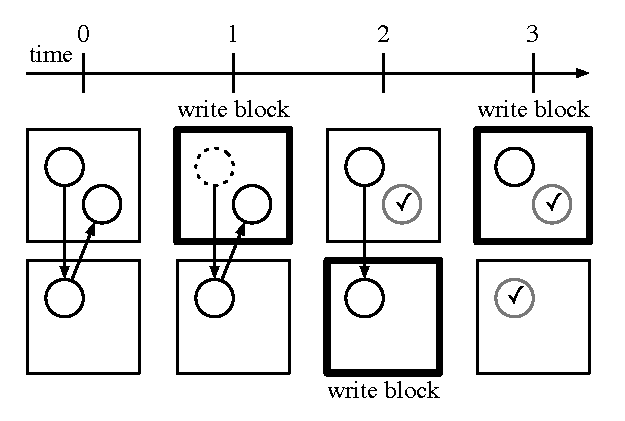
\includegraphics[width=200pt]{rollback_sequence}
%  \caption{\label{fig:rollback} Rolling back change descriptors. Although no
%  cycles are allowed in change descriptor graphs, cycles can exist at the block
%  level which require some change descriptors to be rolled back in order to
%  write the blocks. Here the squares are disk blocks, and dotted circles are
%  rolled back change descriptors. Check marks indicate committed change
%  descriptors.
%}
%\end{figure}
